\documentclass[12pt,border=1pt]{standalone}
\usepackage[T1]{fontenc}
\IfFileExists{newtxtext.sty}{\usepackage{newtxtext,newtxmath}}{\usepackage{mathptmx}}
\usepackage{amsmath,amssymb}
\usepackage[table]{xcolor}
\usepackage{tikz}
\usetikzlibrary{arrows.meta,positioning,fit,calc,decorations.pathreplacing}
\tikzset{blk/.style={draw=black!55,rounded corners=2pt,align=center,font=\footnotesize,inner sep=4pt,minimum height=1.05cm},
         nn/.style={blk,fill=orange!12,draw=orange!70!black},
         lat/.style={blk,fill=blue!8,draw=blue!60!black},
         io/.style={blk,fill=black!3},
         arr/.style={-{Stealth[length=2.2mm]},thick,draw=black!65}}
\definecolor{capblue}{RGB}{47,84,150}
\definecolor{linkblue}{RGB}{17,85,204}
\definecolor{ganttA}{RGB}{11,90,110}
\definecolor{ganttB}{RGB}{20,150,160}
\definecolor{rowhl}{RGB}{253,236,224}
\definecolor{rowhl2}{RGB}{224,244,238}
\begin{document}
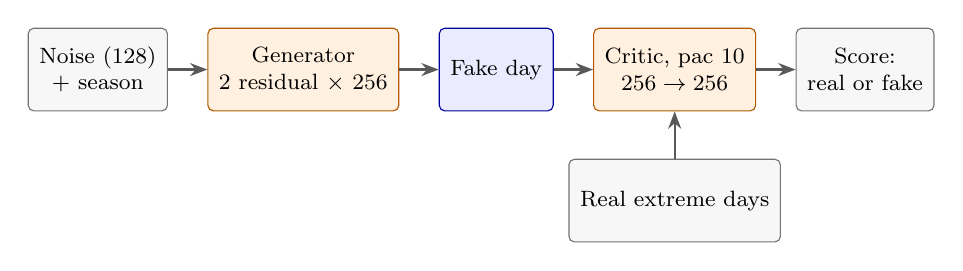
\begin{tikzpicture}[node distance=5mm]
\node[io] (z) {Noise (128)\\+ season};
\node[nn,right=of z] (g) {Generator\\2 residual $\times$ 256};
\node[lat,right=of g] (f) {Fake day};
\node[nn,right=of f] (c) {Critic, pac 10\\$256\to256$};
\node[io,right=of c] (s) {Score:\\real or fake};
\node[io,below=6mm of c] (r) {Real extreme days};
\foreach \a/\b in {z/g,g/f,f/c,c/s} \draw[arr] (\a) -- (\b);
\draw[arr] (r) -- (c);
\end{tikzpicture}
\end{document}
